\documentclass[fontset=windows]{ctexart}
\usepackage{amsmath,amssymb}
\usepackage{fontspec}
\usepackage{graphicx}
\usepackage{subfigure}
\usepackage{fullpage}
\usepackage{setspace}
\usepackage{verbatim}
\usepackage[colorlinks,linkcolor=blue]{hyperref}
\usepackage{listings}
\usepackage{xcolor}
\usepackage{xeCJK}
\setmainfont{Times New Roman}
% \setCJKmainfont{SimSun}
\setCJKmonofont{Consolas}
\newCJKfontfamily[kai]\kaiti{KaiTi}
\newCJKfontfamily[HWkai]\hwkaiti{STKaiti}
% \newCJKfontfamily[hei]\heiti{SimHei}
% \newCJKfontfamily[song]\songti{SimSun}
\newfontfamily\consolas{Consolas}
\lstset{
    columns=fixed,       
%    numbers=left,                                        % 在左侧显示行号
	frame=none,                                          % 不显示背景边框
	basicstyle=\consolas,
    backgroundcolor=\color[RGB]{245,245,244},            % 设定背景颜色
    keywordstyle=\consolas\color[RGB]{40,40,255},                 % 设定关键字颜色
	numberstyle=\consolas\color[RGB]{0,255,0},           % 设定行号格式
    commentstyle=\hwkaiti\consolas\color[RGB]{0,96,96},                % 设置代码注释的格式
    stringstyle=\consolas\color[RGB]{255,0,0},   % 设置字符串格式
    showstringspaces=false,                              % 不显示字符串中的空格
    language=c++,                                        % 设置语言
}
\onehalfspacing
\title{\bf\huge 计算机图形学基础教程}
\author{清华大学\ 计算机科学与技术系}
\date{\today}

\begin{document}
\maketitle

%\hwkaiti{}
% \renewcommand{\contentsname}{目录}
% \renewcommand{\figurename}{图 }

\tableofcontents

\newpage

\section{OpenGL 教程}

\subsection{OpenGL 概述}

\emph{}

OpenGL 是一套开放标准的跨平台高性能图形 API,可以帮助使用者快速创建高性能图形应用程序。
自发布以来,OpenGL 由于其开放性、易用性、可移植性等诸多优点,被广泛地应用在各类图形软件中。

OpenGL的前身是美国硅图公司(Silicon Graphics Inc, SGI)为其图形工作站开发的专有图形接口 IRIS GL。
由于当时不同组织设计的图形硬件设备使用的接口都是专有化的,
图形软件开发者不得不为每种硬件编写不同的代码,
这使得开发图形软件的成本十分昂贵。
20世纪90年代初,SGI 公司意识到了可移植性的重要性,针对性地修改了 IRIS GL 的接口,
移除了其中与特定系统相关的内容,将其作为开放标准发布,即 OpenGL。

1992 年 OpenGL 1.0 版本发布,之后历经二十余年的发展,迭代至今已发布至 4.6 版本。
其维护组织也从 OpenGL 架构审查委员会(OpenGL ARB)转为 Khronos Group。
随着计算机图形硬件的发展,现代图形 API 也逐渐向更加通用的计算发展。
如今,OpenGL 已经几乎停止更新,Khronos Group于2015年发布了其继任者 Vulkan API 标准。
新的标准采用了更底层,更灵活的接口设计,更加适应现代的程序开发模式。
但由于新的接口标准过于复杂,涉及到许多硬件资源的管理问题,对于图形学学习者并不够友好。
OpenGL 在图形应用方面提供了足够强的通用性,并保持着足够好的易用性,
因此其依然是许多情况下最合适的选择。

\subsection{OpenGL 开发环境搭建}

\subsubsection{OpenGL 库}

\emph{}

由于 OpenGL 是一个开放标准,
这使得其接口函数的实现是由不同的图形硬件厂商(如:NVIDIA,AMD,Intel,等)
通过各自的硬件驱动程序提供的。

这样的情况导致许多初学者找不到调用 OpenGL 的方法,因为并不存在一个叫做 OpenGL 的库。
想要调用 OpenGL 函数,必须先从硬件驱动程序中提取出 OpenGL 函数接口。
但由于硬件厂商可能存在不同,驱动程序的位置也往往是不确定的,这给开发者带来了很大的困扰。
针对这个问题,诞生了许多第三方库。
这些第三方库可以帮助开发者完成 OpenGL 环境的创建以及接口函数的提取,
它们往往本身只提供少量几个额外的专有接口用于初始化等操作,
且这些第三方库本身也是跨平台且开源的,
因此可移植性不会受到影响,可以放心使用。
OpenGL 支持多种常见的编程语言,如:C,C++,Python,Java,等。
本章内容只介绍其在 C/C++ 环境中的使用方法,其他语言的接口定义与 C/C++ 版本基本一致,
如有需要可以非常方便地进行迁移。

本章接下来的教程将使用 GLFW 和 GLAD 这两个第三方库作为样例。
这两个库到本书修订时维护状态较好,故推荐优先选择。
其中 GLFW 负责窗口及环境创建,GLAD 负责提取 OpenGL 接口函数。
其他具有相同功能的库,如:GLUT,GLEW,等,使用方法大同小异,故不再一一介绍。

\subsubsection{Windows 环境搭建}

\label{sec-gl:build-windows-env}

在 Windows 系统上的 OpenGL 环境搭建推荐选择 Visual Studio IDE,
本段将以 Visual Studio 2022 Community 为平台演示基于 GLFW 和 GLAD 的 OpenGL 开发环境搭建流程。

1. 获取 GLFW

前往 \href{https://www.glfw.org/}{GLFW 官方网站 (https://www.glfw.org/)},
从网站主页顶部导航栏进入 “Download(下载)” 页面,
找到 “Windows pre-compiled binaries(Windows 预编译二进制文件)” 部分,
下载你所要编译的程序的位数(注意,不是操作系统位数,而是你要生成的应用程序位数)的版本的文件。
现代的操作系统和应用程序一般都已升级到 64 位,故此处以 64 位版本为例,
点击 “64-bit Windows binaries(64位 Windows 二进制文件)” 按钮,
即可下载得到一个包含 GLFW 最新版本头文件,及支持各种 Windows 平台编译工具链的链接库文件的压缩包。
将该压缩包解压后先保存在一个位置,以方便之后使用。


\begin{figure}[htbp]
    \centering
    
\includegraphics[width = 0.5\linewidth]{imgs/sec 2.2/glfw-download-page.png}
    \centering
    \caption{本书修订时 GLFW 下载页面布局}
    \label{fig-gl:glfw-download-page}
\end{figure}


2. 获取 GLAD

前往 \href{https://glad.dav1d.de/}{GLAD 官方网站(https://glad.dav1d.de/)},
可以看到一个配置页面,这个页面是配置用来生成适用于不同平台的 GLAD 库文件信息的。
对于个人计算机开发环境,我们只需要将 “API-gl” 一栏选择为 “Version 4.6(本书修订时的最新版本)”,
Profile 一栏选择为 “Core”,如图 \ref{fig-gl:glad-generate-settings} 所示,其他选项保留默认设置,然后点击右下角的 “GENERATE” 按钮,
即可获得合适的 GLAD 版本(本书修订时,点击 “GENERATE” 按钮后,页面会跳转到一个资源列表页面,下载其中的压缩包即可)。
下载到的 GLAD 库包含一个 include/ 文件夹和一个 src/ 文件夹,
分别存放有调用 GLAD 所需要的头文件以及对应的源码。
GLAD 不需要任何形式的链接库,只需要在引用其头文件后,
将其源码加入项目工程即可使用。

\begin{figure}[htbp]
    \centering
    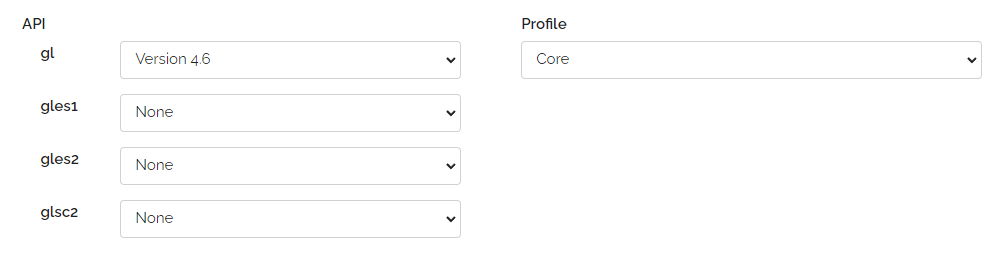
\includegraphics[width = 0.7\linewidth]{imgs/sec 2.2/glad-generate-settings.png}
    \centering
    \caption{GLAD 生成配置(以本书修订时的情况为参考)}
    \label{fig-gl:glad-generate-settings}
\end{figure}

3. 创建 Visual Studio 项目

在进行这一步之前,请先确定系统中已经安装好 Visual Studio, C++ 语言支持,以及 “Windows SDK”,
因为最新版本的 Visual Studio 可以动态配置支持的语言以及拓展工具,
如没有安装 C++ 语言支持,或没有安装 “Windows SDK”,则后续步骤可能无法正常进行。

以 Visual Studio 2022 Community 版本为例。
在准备好以上内容后,进行以下步骤:

- 打开 Visual Studio

- 选择 “创建新项目”

- 选择 “Windows 桌面向导”

- 为项目起一个名称,并选择保存位置,点击 “创建”

- 选择 “控制台应用程序”,并勾选 “空项目”,点击 “确定” 完成项目创建

在项目创建完成后,Visual Studio 会自动打开新创建的项目。
此时,在 “解决方案资源管理器” 中可以看到整个项目的组织结构。
右键点击其中的 “源文件”,依次点击 “添加”-“新建项”;
在弹出的窗口中选择 “C++文件(.cpp)”,
编辑文件名称(如 “main.cpp”),并点击右下角的 “添加”,
即可为新创建的空项目添加一个空的源文件。

在这个新创建的源文件中,可以尝试编写一个 “Hello, World” 程序,按 F5 编译运行,以测试基础环境是否配置正确。

Visual Studio 的功能非常强大,可以配置的选项十分繁复,此处特别提醒:在顶部导航栏可以选择生成应用程序的模式。
Visual Studio 2022 默认为 “Debug-x64”,其中 “Debug” 表示以调试模式编译,
“x64” 表示生成 64 位应用程序。“Debug” 模式默认不开启任何优化,
因此生成的程序运行速度非常慢,如果希望编译高效率的程序,可以将此选项改为 “Release”。
注意,更早版本的 Visual Studio 可能默认目标平台为 “x86”,即 32 位应用程序,
需要手动修改为 “x64” 以适配教程中默认采用的 64 位链接库。

4. 将 OpenGL 库添加到项目中

在进行这一步之前,建议将下载好的 GLFW 和 GLAD 文件移动到项目文件夹中,
以确保项目在迁移到其他设备上时可以正常工作。

为了在编译应用程序时,编译工具能够正确地找到两个第三方库的相关文件,
需要向 Visual Studio 项目添加第三方库的头文件包含目录以及库目录信息,
并将需要用到的静态链接库添加到链接器的配置中。

具体的操作方法为:

在 Visual Studio 窗口顶部导航栏中选择 “项目”-“XXX 属性”(XXX 替换为你的项目名称),
弹出项目属性页。

在属性页顶部首先选择好对应的生成配置,
然后在左侧配置属性中选择 “VC++目录”,
在右侧找到 “包含目录” ,将 GLFW 和 GLAD 文件包中 include/ 目录的路径添加到该项的值中。
再在右侧找到 “库目录” ,将 GLFW 文件包中对应编译工具版本的目录路径添加到该项的值中,
例如,Visual Studio 2022 应选择 “your-glfw-path/lib-vc2022”。

在目录配置完成后,在左侧配置属性中选择 “链接器”-“输入”,
在右侧找到 “附加依赖项”,将 “glfw3.lib” 添加到该项。

最后,保存修改的信息并关闭项目属性页,回到 “解决方案资源管理器”,
右键“源文件”-“添加”-“现有项”,找到 GLAD 文件包中的 src/ 目录,
将其中的 glad.c 文件添加到项目中。

至此,Windows 平台上的 OpenGL 环境配置完毕。
请跳转到 \ref{sec-gl:creating-opengl-window} 节继续阅读。

\subsubsection{Linux 环境搭建}

本节以 Ubuntu-20.04 版本为例,演示在 Linux 平台上的 OpenGL 环境搭建方法。
用于其他 Linux 发行版的方法
可以参考其中共同的部分,
并将和 Ubuntu 系统软件包管理相关的操作替换成对应系统的软件包管理操作。
在搭建 Linux 平台环境之前,请确保所使用的 Linux 平台包含有窗口服务,
否则程序无法正常运行。
一般桌面端的 Linux 发行版都满足此条件,
而服务器端则可能不支持。

1. 获取 GLFW

不同于 Windows 平台,由于 Linux 平台不同发行版之间存在或多或少的差异,
很难提供一套统一的预编译二进制文件。
故,在 Linux 平台上使用 GLFW 库需要通过其开源代码自行编译静态链接库文件。

首先,与 Windows 平台相同,
前往\href{https://www.glfw.org/}{GLFW 官方网站 (https://www.glfw.org/)}
的下载页下载所需的文件。
点击 “Source package(源代码包)” 按钮,获得 GLFW 源代码的压缩包并解压。
进入解压后的文件目录,可以看到一个 CMake 工程的文件结构。

在 GLFW 目录下运行以下指令,以编译安装 GLFW 库文件到系统库目录。

\begin{lstlisting}[language=bash]
sudo apt update
sudo apt install g++ cmake xorg-dev libglu1-mesa-dev
mkdir build
cd build
cmake ..
make
sudo make install
\end{lstlisting}

如未能成功运行以上指令,
可能是系统所使用的软件包管理器不同,
或是缺少一些未被上述指令考虑在内的依赖包,
亦或是权限问题,可以根据问题提示自行搜索解决方案。

2. 获取 GLAD

获取 GLAD 库文件包的方法与 Windows 平台相同,请参考 \ref{sec-gl:build-windows-env} 节对应部分内容。

3. 创建项目代码

在上述操作完成后,在一个合适的位置创建一个项目目录,以下将使用 “project-path/” 代表项目目录。
在创建项目目录后,在项目目录中创建 include/ 目录, makefile 文件及源文件 main.cpp。
然后,将 GLFW 和 GLAD 文件包中的 include/ 目录下的内容复制到 project-path/include/ 目录下;
同时,将 GLAD 文件包中 src/目录下的 glad.c 文件复制到 project-path/ 目录。

此时,项目目录下的文件结构应该如下所示:

\begin{lstlisting}
project-path
├── glad.c
├── include
│   ├── glad
│   │   └── glad.h
│   ├── GLFW
│   │   ├── glfw3.h
│   │   └── glfw3native.h
│   └── KHR
│       └── khrplatform.h
├── main.cpp
└── makefile
\end{lstlisting}

最后,编辑 makefile 文件,写入如下内容

\begin{lstlisting}[language=make]
main: main.cpp glad.c
    g++ main.cpp glad.c -Iinclude -o main -m64 -lglfw3 -lX11 -ldl -pthread
\end{lstlisting}

完成后,即可通过在项目目录下运行如下指令进行程序的编译和运行。

\begin{lstlisting}[language=bash]
make
./main
\end{lstlisting}

\subsubsection{创建 OpenGL 窗口}

在配置好开发环境后,将源文件编写为如下内容,然后编译运行。

\begin{lstlisting}[language=c++]
#include <glad/glad.h>
#include <GLFW/glfw3.h>
#include <iostream>

int main(void)
{
    GLFWwindow* window;

    /* 初始化 GLFW 库 */
    if (!glfwInit())
        return -1;

    /* 创建窗口 */
    window = glfwCreateWindow(640, 480, "Hello World", NULL, NULL);
    if (!window)
    {
        glfwTerminate();
        return -1;
    }

    /* 将窗口设置为当前上下文 */
    glfwMakeContextCurrent(window);

    /* 初始化 GLAD 库,在这一步之后才能调用 glXXX 函数 */
    if (!gladLoadGLLoader((GLADloadproc)glfwGetProcAddress))
    {
        glfwTerminate();
        return -1;
    }

    /* 显示设备信息以及 GL 版本 */
    std::cout << "GPU:         " << glGetString(GL_RENDERER) << std::endl;
    std::cout << "GPU Vendor:  " << glGetString(GL_VENDOR) << std::endl;
    std::cout << "GL Version:  " << glGetString(GL_VERSION) << std::endl;

    /* 消息循环 */
    while (!glfwWindowShouldClose(window))
    {
        /* 在这里实现渲染代码 */
        glClearColor(0.6, 0.7, 0.8, 1.0);
        glClear(GL_COLOR_BUFFER_BIT);

        /* 交换缓冲 */
        glfwSwapBuffers(window);

        /* 处理窗口消息 */
        glfwPollEvents();
    }

    glfwTerminate();
    return 0;
}
\end{lstlisting}

如果所有配置都没有错误,即可看到一个 $640\times 480$ 的窗口,如图\ref{fig-gl:hello-window}所示。
同时,控制台会显示出使用的 GPU 设备型号,制造商,以及支持的 OpenGL 版本信息。
如下所示:

\begin{figure}[htbp]
    \centering
    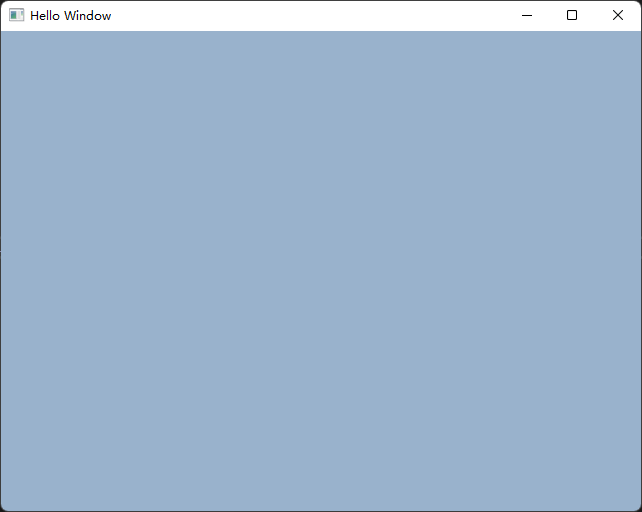
\includegraphics[width = 0.5\linewidth]{imgs/sec 2.4/hello-window.png}
    \caption{代码正常运行时应当显示的窗口}
    \label{fig-gl:hello-window}
\end{figure}

\begin{lstlisting}
GPU:         NVIDIA GeForce RTX 3090/PCIe/SSE2
GPU Vendor:  NVIDIA Corporation
GL Version:  4.6.0 NVIDIA 497.29
\end{lstlisting}

以此为例:
第一行显示使用的显卡名称;
第二行显示显卡厂商;
第三行显示 OpenGL 版本,第一个版本号表示 OpenGL 接口支持的版本,
第二个版本号表示显卡驱动的版本。

如果 OpenGL 未能运行在正确的设备上,
比如:对于同时具有集成显卡和独立显卡的系统,OpenGL 选择了低性能的集成显卡。
则可能需要在操作系统中手动设置图形硬件优先级。
如果发现支持的 OpenGL 版本过低,可能是驱动程序过于老旧,
此时应该及时更新最新的驱动程序。
如更新驱动程序后问题依旧不能解决,
则可能是显卡设备本身过于老旧,无法支持新版本的接口,
但一般不会发生此类情况。

\label{sec-gl:creating-opengl-window}

如果到此处所有功能运行正常,则可顺利进入图形绘制部分代码的编写。

\subsection{绘制三角形}

现代图形 API 普遍以三角形为基本元素进行绘制。
一般来说,在成功创建窗口后,
接下来要做的就是绘制一个三角形,
由此打开通往高性能图形应用开发的大门。
因此 “Hello, Triangle” 就相当于图形领域的 “Hello,World”,
成为了使用任何图形接口进行开发的第一课。

\subsubsection{顶点缓冲}

想要绘制一个三角形,
首先需要定义出这个三角形的样子。
而定义一个三角形最简单的方法就是给出其三个顶点的位置。
在二维空间中,三角形的一个顶点可以用一个二元组表示,
在三维空间中,三角形的一个顶点可以用一个三元组表示;
但这不是顶点在现代化的图形 API 中真正的表示方法。
现代图形 API 普遍用一个四元组表示一个三维坐标,
这种表示法被称作 “齐次坐标”,
额外的那个维度可以理解为坐标的 “缩放反比”。
例如,一个四元组 $(x,y,z,w)$ 所表示的三维坐标为
$(\frac{x}{w},\frac{y}{w},\frac{z}{w})$。
一般情况下,$w=1$;而当 $w=0$ 时,该四元组表示 $(x,y,z)$ 向量。
这种表示法可以带来诸多好处,这部分内容将在 \ref{sec-gl:projection-matrix} 节详细展开。

除了顶点的位置信息之外,一个顶点可能还会包括颜色,法向量,纹理坐标等服务于渲染的其他信息。
为了简化绘制复杂性,目前阶段对于一个顶点只考虑其位置和颜色信息。
这两个信息分别可由一个四元组表示,位置信息为齐次坐标 $(x,y,z,w)$,
而颜色信息为三通道颜色加上 alpha 通道 $(r,g,b,a)$。
于是,可以用如下方式定义一个三角形的三个顶点的数据:

\begin{lstlisting}[language=c++]
float vertex_buffer[3][8] = {
    { 0.0f,  0.5f, 0.0f, 1.0f, 1.0f, 0.0f, 0.0f, 1.0f},
    { 0.5f, -0.5f, 0.0f, 1.0f, 0.0f, 1.0f, 0.0f, 1.0f},
    {-0.5f, -0.5f, 0.0f, 1.0f, 0.0f, 0.0f, 1.0f, 1.0f},
};
\end{lstlisting}

其中每一个八元组的前四个元素表示 $(x,y,z,w)$,后四个元素表示 $(r,g,b,a)$。
对于在二维平面上绘制的情况,坐标的第三维度暂时没有意义,故置为 $0$;
alpha 通道默认为 $1$。

定义好三角形的顶点数据后,需要将这些定点信息传入 GPU 用于绘制。
但 CPU 与 GPU 之间的通信是一个开销非常大的操作,
为了提高应用程序的执行效率,
需要尽可能减少 CPU 与 GPU 之间的通信次数。
因此,为了避免每一帧的绘制都需要将绘制过程的资源从 CPU 端传到 GPU 端,
在现代化的图形渲染接口都会提供 GPU 端的缓冲区机制。
缓冲区本质是显存中的一块区域,可以像内存一样存取数据。
不同点是,显存对于 GPU 访问响应速度非常快,对于 CPU 访问响应速度非常慢,而内存反之。
缓冲本身仅用于保存数据,而不关心数据本身的含义,
只有将其绑定到渲染流水线的不同部分时,缓冲才会被赋予不同的意义。
在绘制三角形时,需要先将三角形的顶点信息存入一个缓冲区,
以供渲染流水线调用,这种缓冲区被称作顶点缓冲。

在现代 OpenGL 中,缓冲区需要由程序员手动创建,
赋值。这些操作需要用到如下函数:

\begin{lstlisting}[language=c++]
void glCreateBuffers( GLsizei n, GLuint * buffers );

void glNamedBufferData(
    GLuint buffer,
    GLsizei size,
    const void *data,
    GLenum usage
    );

void glNamedBufferSubData(
    GLuint buffer,
    GLintptr offset,
    GLsizei size,
    const void *data
    );
\end{lstlisting}

glCreateBuffers 用于创建缓冲区对象,并返回创建所对象的标识符。

OpenGL 的对象管理机制并非通过接口类实现,
而是通过标识符实现。
所谓标识符,即一个无符号 32 位整数。
需要对某一对象进行操作时,在调用函数时传入对应的标识符即可表明所操作的对象是哪一个。
因此,在创建某一种对象时,需要调用对应的 glCreate***s 函数获取对应的标识符。
这类函数的调用方法几乎一致,
函数参数为一个整数 $n$ 和一个指向接受标识符的地址空间的指针 $buffers$。
函数会在 $buffers$ 指向的地址空间的前 $n$ 个位置写入 $n$ 个不同的标识符,
指向新创建的 $n$ 个对象。

在只创建一个标识符时,可以这样调用:

\begin{lstlisting}[language=c++]
uint32_t vertex_buffer_object;
glCreateBuffers( 1, &vertex_buffer_object );
\end{lstlisting}

在创建多个标识符时,以 5 个为例,可以这样调用:

\begin{lstlisting}[language=c++]
uint32_t vertex_buffer_objects[5];
glCreateBuffers( 5, vertex_buffer_objects );
\end{lstlisting}

注意,在 OpenGL 函数定义中有许多以 GL 开头的类型,
这是 OpenGL 为了避免在不同平台上原生类型数据长度不统一而设计的。
为了更好地兼容与其他编程库并用时的类型统一性,
建议使用 C/C++ 标准的定长类型替代 GL 类型。
表 \ref{tab-gl:opengl-type} 是一个常用类型之间的简要对照表。

\begin{table}[htbp]
    \centering
    \begin{tabular}{|l|l|l|}
        \hline
        OpenGL 类型 & 类型实质 & 标准类型\\
        \hline
        GLint & 32 位整型 & int32\_t\\
        \hline
        GLuint & 32 位无符号整型 & uint32\_t\\
        \hline
        GLint64 & 64 位整型 & int64\_t\\
        \hline
        GLuint64 & 64 位无符号整型 & uint64\_t\\
        \hline
        GLbyte & 8 位整型 & int8\_t\\
        \hline
        GLubyte & 8 位无符号整型 & uint8\_t\\
        \hline
        GLenum & 32 位无符号整型 & uint32\_t\\
        \hline
        GLsizei & 32 位整型 & int32\_t\\
        \hline
        GL*ptr & 64 位整型 & int64\_t\\
        \hline
        GLchar & 8 位整型(字符) & int8\_t (char)\\
        \hline
        GLboolean & 8 位无符号整型 & uint8\_t\\
        \hline
        GLfloat & 32 位浮点数(单精度浮点数) & float\\
        \hline
        GLdouble & 64 位浮点数(双精度浮点数) & double\\
        \hline
    \end{tabular}
    \caption{OpenGL 类型对照表}
    \label{tab-gl:opengl-type}
\end{table}

在创建缓冲区对象后,需要使用 glNamedBufferData 函数对新的缓冲区对象创建对应的缓冲区。
函数参数 buffer 表示需要进行创建缓冲区操作的缓冲对象的标识符;
size 表示所要创建的缓冲区的长度,以字节为单位;
data 表示指向用于初始化缓冲区数据的指针,置为 nullptr 则表示不初始化缓冲区的数据;
usage 表示该缓冲区的使用方式特征,需要传入 OpenGL 标准定义的宏。

若想创建一个用于绘制三角形的顶点缓冲区,可以这样调用:

\begin{lstlisting}
glNamedBufferData(
    vertex_buffer_object,
    sizeof(vertex_buffer),
    nullptr,
    GL_STATIC_DRAW);
\end{lstlisting}

其他参数在之前的内容中出现过,不再一一解释。
函数的最后一个参数 GL\_STATIC\_DRAW 表示该缓冲区的数据不会经常被 CPU 写入,
会被经常用于 GPU 端的绘制操作。

这个位置的参数可以看做由两部分组成,首先是表示被访问频率的第一部分,取值有:

1. STATIC;表示很少被 CPU 修改,但会频繁地被 GPU 使用。

2. DYNAMIC;表示经常被 CPU 修改,也会频繁地被 GPU 使用。

3. STREAM;表示很少被 CPU 修改,也只会被 GPU 使用有限的几次,在图形应用中很少会用到。

其次是表示 GPU 端使用方式的第二部分,取值有:

1. DRAW;表示被 CPU 修改,用于 GPU 端的绘制。

2. COPY;表示会被 GPU 端修改,用于 GPU 端的绘制,在图形应用中很少会用到。

3. READ;表示会被 GPU 端修改,用于向 CPU 返回数据,在图形应用中很少会用到。

在常见的 OpenGL 使用情形中,一般将不会每一帧都变换的资源设置为 GL\_STATIC\_DRAW,
将每一帧都很可能发生变化的资源设置为 GL\_DYNAMIC\_DRAW。
此外,这个参数仅表示所创建的缓冲区的使用特征的提示信息,
硬件驱动可能会根据这个参数对数据处理流程做一些优化,
但这个参数不会影响创建出的缓冲区的功能性,仅可能影响缓冲区在执行不同操作时的效率。

在创建好缓冲区后,需要调用 glNamedBufferSubData 函数将 CPU 端的数据上传到缓冲区。
初次上传可以在调用 glNamedBufferData 时完成,但后续的更改需要依赖这个函数。调用方法如下:

\begin{lstlisting}[language=c++]
glNamedBufferSubData(
    vertex_buffer_object,
    0,
    sizeof(vertex_buffer),
    vertex_buffer);
\end{lstlisting}

其中,0 表示缓冲区目标上传位置的偏移量,
sizeof(vertex\_buffer) 表示上传数据的长度,
vertex\_buffer 为 CPU 端数据的起始位置指针。
所示函数调用语句表示把所有顶点数据全部复制到缓冲区中。

如想验证数据是否成功地被复制到缓冲区中,
可以通过 glGetNamedBufferSubData 函数将数据从缓冲区中取回。
调用方法如下:

\begin{lstlisting}
float vertex_buffer_copy[3][8];
glGetNamedBufferSubData(
    vertex_buffer_object,
    0,
    sizeof(vertex_buffer_copy),
    vertex_buffer_copy);
\end{lstlisting}

glGetNamedBufferSubData 函数参数含义与 glNamedBufferSubData 基本一致,
区别在于数据流向相反。所示代码将缓冲区中数据复制到了与 CPU 端原数据无关的区域
vertex\_buffer\_copy。
可以通过简单的输入输出手段查看 vertex\_buffer\_copy 中的数据与 vertex\_buffer
是否相同验证数据拷贝是否成功。

\subsubsection{着色器}

\subsubsection{配置管线}

\subsubsection{完整代码}

\subsection{绘制立方体}

\subsubsection{标准化设备坐标空间}

\subsubsection{投影矩阵}

\label{sec-gl:projection-matrix}

\subsubsection{uniform 变量}

\subsubsection{索引缓冲}

\subsubsection{深度缓冲}

\subsection{纹理贴图}

\subsubsection{加载纹理}

\subsubsection{绘制纹理}

\subsection{光照}

\subsubsection{实现基于 BRDF 的光照}

\subsubsection{绘制阴影}

\subsection{绘制到纹理}

\subsubsection{帧缓冲}

\subsection{更多学习资源}


\end{document}
